\section{INTRODUCTION}
\label{sec:intro}

\begin{figure*}[h!]
    \centering
    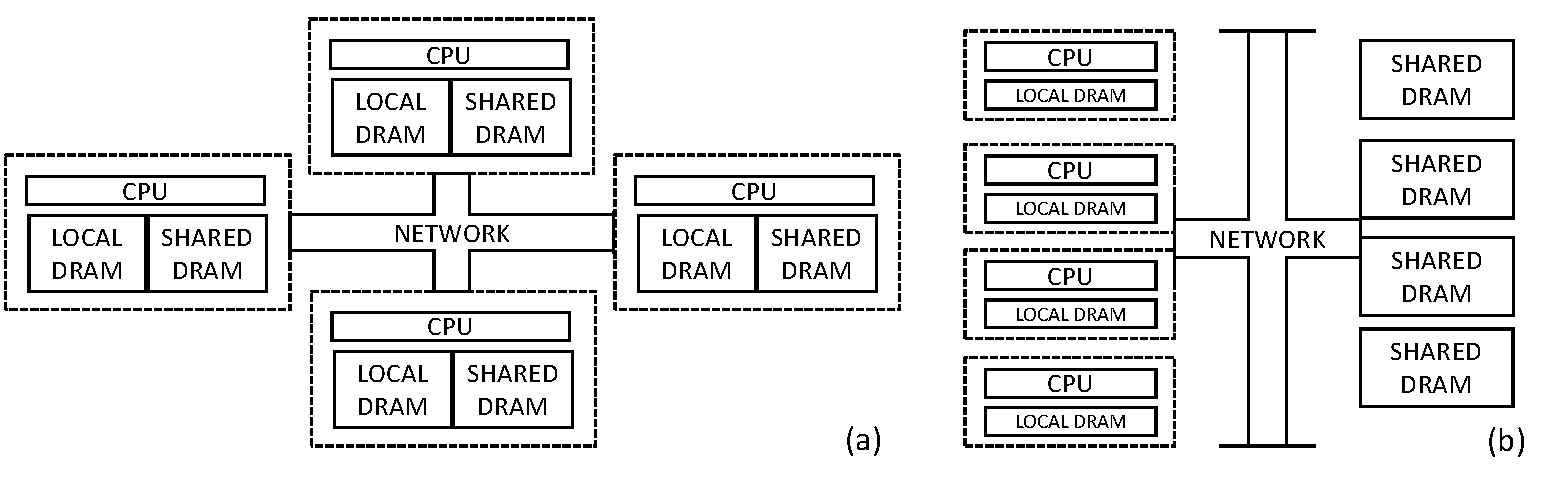
\includegraphics[width=.9\linewidth]{fig/architecture.pdf}
    \caption{(too big?) Shows (a) software-disaggregated architecture where disaggregated memory is pooled from 
    traditional servers as opposed to the (b) hardware-disaggregated
    design where most memory is decoupled in hardware.}
    \label{fig:architecture}
\end{figure*}

With the tremendous growth of computing in the past two decades, 
applications has become both data-intensive and latency-
sensitive, which gave rise to in-memory computing in lieu 
of going to the disk. This led to memory-intensive 
applications whose memory needs on a server outweigh the 
processor needs, introducing a skew in resource usage.
However, traditional servers come with fixed processor 
and memory resources that does not allow dynamically
resizing memory. Traditionally, this was solved by swapping 
to disk but disk speeds were really slow compared to memory 
affecting performance. 

At the same time, the diversification of computing usecases 
introduced a high heterogeneity of applications (e.g., cloud 
computing) with varying memory needs in proportion to 
the CPU, leaving some of the traditional servers in a data center  
with underutilized memory and others with not enough; the result
being inefficient memory utilization in the cluster and hence,
increased cost of ownership. Decoupling memory would allow 
applications to be more elastic in their memory usage and 
improve the memory utilization of the cluster at the same time.
Memory disaggregation involves such (logical or physical) 
decoupling of memory resources in a cluster from other 
(processor) resources. 
% \anil{there are other benefits to memory disaggregation...}

\mc{Scoping}
An obvious way to alleviate memory pressure is to build a 
distributed application that runs on multiple nodes and 
adjust itself to the memory restrictions on the individual 
nodes. Indeed, there is a lot of work here that focus on building 
performant distributed applications, like the in-memory 
data stores (e.g., RAMCloud, RDMA-based KVS papers, etc.\todo{cite some}). 
However, these solutions are specific to those applications and 
do not generalize. However, we are looking for general 
platforms (rather than individual applications) that provide 
(somewhat) generic, low-level interfaces targeting a wide 
spectrum of applications and allow them to efficiently utilize 
the entire memory of the cluster. Some of the earlier 
systems that provided such mechanisms include the remote 
swapping systems~\cite{gms,cashmere} that transparently moved 
around the pages of virtual memory subsystem in the cluster,
and distributed shared memory systems~\cite{treadmarks,dsm1}
that did the same behind a global virtual address space.
\anil{Remote memory draws from this lesson and avoids the hard problem of sharing: its goal is not to implement shared memory. In fact, remote memory need not be shared at all: it can be used to store private pages to extend local memory or to safeguard data remotely. Or it can provide a different form of sharing: we envision non-simultaneous sharing of remote memory, whereby a host stops using the data before another node starts (e.g., in different phases of map-reduce).}

\anil{There are many ways for a machine to store data remotely,
such as using key-value storage systems (e.g., [16, 17, 28, 36]), tuples [14], distributed objects [45], files, database systems, and RDMA [4, 5]. While effective, these abstractions are fundamen- tally different from the abstraction of memory accessed via}
Traditional way of memory disaggregation is to pool/track  
unused memory across the cluster in software 
and use it to complement memory on the memory-hungry servers.
This is still popular with work on remote swapping systems 
continuing to this day~\cite{infiniswap,fastswap,zswap,leap}.
The other, more recent-style is to disaggregate the memory 
in hardware and is available to all the compute nodes through
the network~\cite{legoos}. In both cases, building a system 
that exposes and manages such disaggregated memory face very 
similar design challenges. First, the system should decide on
the right interface to expose this memory; for example,
to either be transparent and avoid any application changes, 
or to be more expressive to provide richer functionality and 
allow app optimizations. Remote access latencies are still an 
order-of-magnitude worse than local, so the system should 
decide on performance optimizations like caching or at least,
enable applications to implement their optimizations. 
While providing reasonable programming model and performance
for a wide set of applications, it should also work towards 
efficiently managing the cluster memory behind the scenes and 
maintain good utilization - our goal in the first place.

In this report, we explore in detail, the above design 
challenges of building a system for disaggregated memory, 
and some more that is expected of a holistic system e.g., 
fault tolerance, reliability, security and isolation, etc.
through the lens of recent disaggregated/far memory systems.
~\cite{infiniswap,zswap,leap,fastswap,legoos,kona,aifm,semeru,
remregions,literdma}. Through this analysis, we hope to 
highlight the trade-offs involved with various design 
considerations and challenges left for widespread adoption.
We end with a discussion on \todo{}.
